%%%%%%%%%%%%%%%%%%%%%%%%%%%%%%%%%%%%%%%%%
% Beamer Presentation
% Computer Architecture
% Term Paper Presentation: Turing Architecture
%
% Gahan M. Saraiya
% 18MCEC10
%
%%%%%%%%%%%%%%%%%%%%%%%%%%%%%%%%%%%%%%%%%
%----------------------------------------------------------------------------------------
%       PACKAGES AND OTHER DOCUMENT CONFIGURATIONS
%----------------------------------------------------------------------------------------
\documentclass[xcolor=x11names,table]{beamer}

%\usepackage{beamerthemeCambridgeUS}  % CambridgeUS theme
% for themes, etc.
%\mode<presentation>
%{ \usetheme{boxes} }

\usetheme{EastLansing}
\usepackage{float}  % perfect fit graphic with command [H]
%\usepackage{tabularx}  % alternate to tabular to use X to wrap column data properly
%\usetheme{Antibes}
\usepackage{hyperref}

%package for timeline
\usepackage[utf8]{inputenc}
\usepackage[english]{babel}
\usepackage[TS1,T1]{fontenc}
\usepackage{fourier, heuristica}
\usepackage{array, booktabs}
\usepackage{longtable}
\usepackage{makecell}
%\usepackage[x11names]{xcolor}
%\usepackage{caption}
%\DeclareCaptionFont{blue}{\color{LightSteelBlue3}}

\newcommand{\foo}{\color{LightSteelBlue3}\makebox[0pt]{\textbullet}\hskip-0.5pt\vrule width 1pt\hspace{\labelsep}}
\usepackage{times}  % fonts
\usepackage{graphicx, wrapfig} % for graphics

\usepackage{media9}

\usepackage{scrextend}
%colours
\definecolor{lightblue}{rgb}{0.1, 0.1, 0.6}
\definecolor{maroon}{rgb}{0.3, 0.1, 0.7}

\newcommand{\FR}[2]{
	{\textstyle \frac{#1}{#2} }}
\def\RR{\mathbb{R}}
% macros
\newcommand{\hhq}{{\scriptstyle{{\frac{1}{4}}}}}
\newcommand\hf{\textstyle{1\over 2 }\displaystyle}
\newcommand\hhf{\scriptstyle{1\over 2 }\displaystyle}
\newcommand{\erf}{\mathrm{erf}}
\def\h{\textcolor{red}{\mathbf{h}}}
\def\z{\textcolor{maroon}{\mathbf{z}}}
\newcommand{\zave}{\z_{\mathrm{ave}}}
\def\by{\textcolor{lightblue}{\mathbf{y}}}
\def\bv{\textcolor{blue}{\mathbf{v}}}
\def\bx{\textcolor{red}{\mathbf{x}}}
\def\bp{\textcolor{maroon}{\mathbf{p}}}
\makeatother

\renewcommand\theadalign{bc}
\renewcommand\theadfont{\bfseries}
\renewcommand\theadgape{\Gape[4pt]}
\renewcommand\cellgape{\Gape[4pt]}
\newcommand*\tick{\item[\Checkmark]}
\newcommand*\arrow{\item[$\Rightarrow$]}
\newcommand*\fail{\item[\XSolidBrush]}
\usepackage{minted} % for highlighting code sytax
\definecolor{LightGray}{gray}{0.9}

\setminted[text]{
	frame=lines, 
	breaklines,
	baselinestretch=1.2,
	bgcolor=LightGray,
	%	fontsize=\small
}
%----------------------------------------------------------------------------------------
%       Video Stuff
%----------------------------------------------------------------------------------------
\usepackage{media9}
%----------------------------------------------------------------------------------------
%       GRAPH PLOTING CONFIG
%----------------------------------------------------------------------------------------
\usepackage{pgfplotstable}

\usetikzlibrary{backgrounds}
% background color definition from pgfmanual-en-macros.tex
\definecolor{graphicbackground}{cmyk}{0.04,0.02,0.02,0.04}
% key to change color
\pgfkeys{/tikz/.cd,
	background color/.initial=graphicbackground,
	background color/.get=\backcol,
	background color/.store in=\backcol,
}
\tikzset{background rectangle/.style={
		fill=\backcol,
	},
	use background/.style={
		show background rectangle
	}
}

% *** FLOWCHART AND GRAPHS PACKAGES ***
%
\usepackage{tikz}
\usetikzlibrary{snakes,arrows,shapes, shapes.geometric, calc, automata,positioning}
\tikzstyle{startstop} = [rectangle, rounded corners, minimum width=3cm, minimum height=1cm,text centered, trapezium stretches=true, draw=black, fill=red!30]
\tikzstyle{io} = [trapezium, trapezium left angle=70, trapezium right angle=110, minimum width=3cm, trapezium stretches=true, minimum height=1cm, text centered, draw=black, fill=blue!30]
\tikzstyle{process} = [rectangle, minimum width=3cm, minimum height=1cm, text centered, draw=black, trapezium stretches=true, fill=orange!30]
\tikzstyle{decision} = [diamond, minimum width=3cm, minimum height=1cm, text centered, draw=black, trapezium stretches=true, fill=green!30]
\tikzstyle{arrow} = [thick,->,>=stealth]
%----------------------------------------------------------------------------------------
%       CUSTOMIZE BEAMER FOOTER
%----------------------------------------------------------------------------------------
\setbeamertemplate{footline}
{
	\leavevmode%
	\hbox{%
		\begin{beamercolorbox}[wd=.4\paperwidth,ht=2.25ex,dp=1ex,center]{author in head/foot}%
			\usebeamerfont{author in head/foot}\insertshortauthor
		\end{beamercolorbox}%
		\begin{beamercolorbox}[wd=.6\paperwidth,ht=2.25ex,dp=1ex,center]{title in head/foot}%
			\usebeamerfont{title in head/foot}\insertshorttitle\hspace*{3em}
			%			\insertframenumber{} / \inserttotalframenumber\hspace*{1ex}
	\end{beamercolorbox}}%
	\vskip0pt%
}
\makeatletter
\setbeamertemplate{navigation symbols}{}




%----------------------------------------------------------------------------------------
%       Glossaries
%----------------------------------------------------------------------------------------
\usepackage{glossaries}

\makeglossaries
\loadglsentries{glossaries}

%----------------------------------------------------------------------------------------
%       TITLE SECTION
%----------------------------------------------------------------------------------------
\title{Turing Architecture}
\author{Gahan M. Saraiya (18MCEC10)}
\institute{M.Tech (Computer Science and Engineering) 
	\\ Institute of Technology, Nirma University, Ahmedabad}
\date{{\scriptsize November 2018}}

% note: do NOT include a \maketitle line; also note that this title
% material goes BEFORE the \begin{document}

% Recurring Outline for every section, with highlighting
\AtBeginSection[]
{ \begin{frame}<beamer> 
	\frametitle{Outline of Talk}
	\tableofcontents[currentsection]%[pausesections]
\end{frame} }

\hypersetup{
colorlinks=true,
linkcolor=blue,
filecolor=magenta,      
urlcolor=cyan,
pdfauthor={Gahan Saraiya},
pdfcreator={Gahan Saraiya},
pdfproducer={Gahan Saraiya},
}

%----------------------------------------------------------------------------------------
%       BEGIN DOCUMENT
%----------------------------------------------------------------------------------------
\pgfplotsset{compat=1.15}
\begin{document}
\maketitle
%\begin{frame}
%\titlepage
%\end{frame}

\section{Introduction}
\begin{frame}[allowframebreaks]
\frametitle{What is Turing Architecture?}
    \begin{itemize}
    	\item codename for a GPU microarchitecture developed by Nvidia
    	\item Successor of
    	    \href{https://en.wikipedia.org/wiki/Volta_(microarchitecture)}{Volta}
    	\item named after well known mathematician and computer scientist
    	    \href{https://en.wikipedia.org/wiki/Alan_Turing}{Alan Turing}
    	\item the first consumer product with capability of real-time \gls{ray-tracing}
    	\item NVIDIA partnered with Microsoft to enable full RTX support via
    	    \href{https://blogs.msdn.microsoft.com/directx/2018/03/19/announcing-microsoft-directx-raytracing/}{Microsoft’s new DirectX Raytracing (DXR) API}
    	\item TU102 GPU includes \textbf{18.6 billion transistors} fabricated on TSMC’s 12 nm FFN (FinFET NVIDIA) high-performance manufacturing process
    \end{itemize}
    \begin{figure}[H]
    	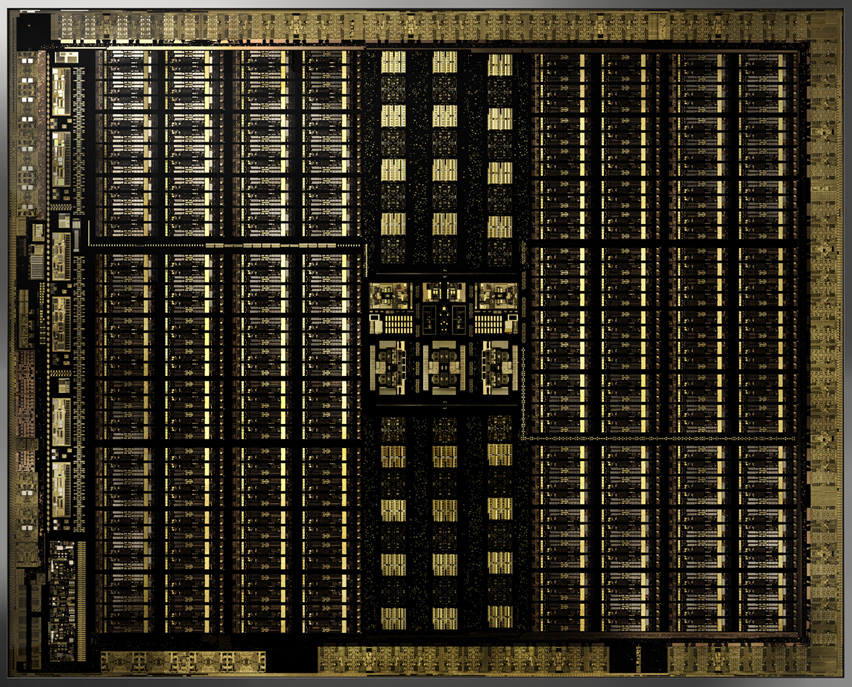
\includegraphics[width=220px]{refs/NVIDIA-Turing-Architecture-TU102}
    	\caption{Turing Architecture in TU102}
    \end{figure}
\end{frame}

%	\usebackgroundtemplate{
%		tikz\node[opacity=0.1]{
%		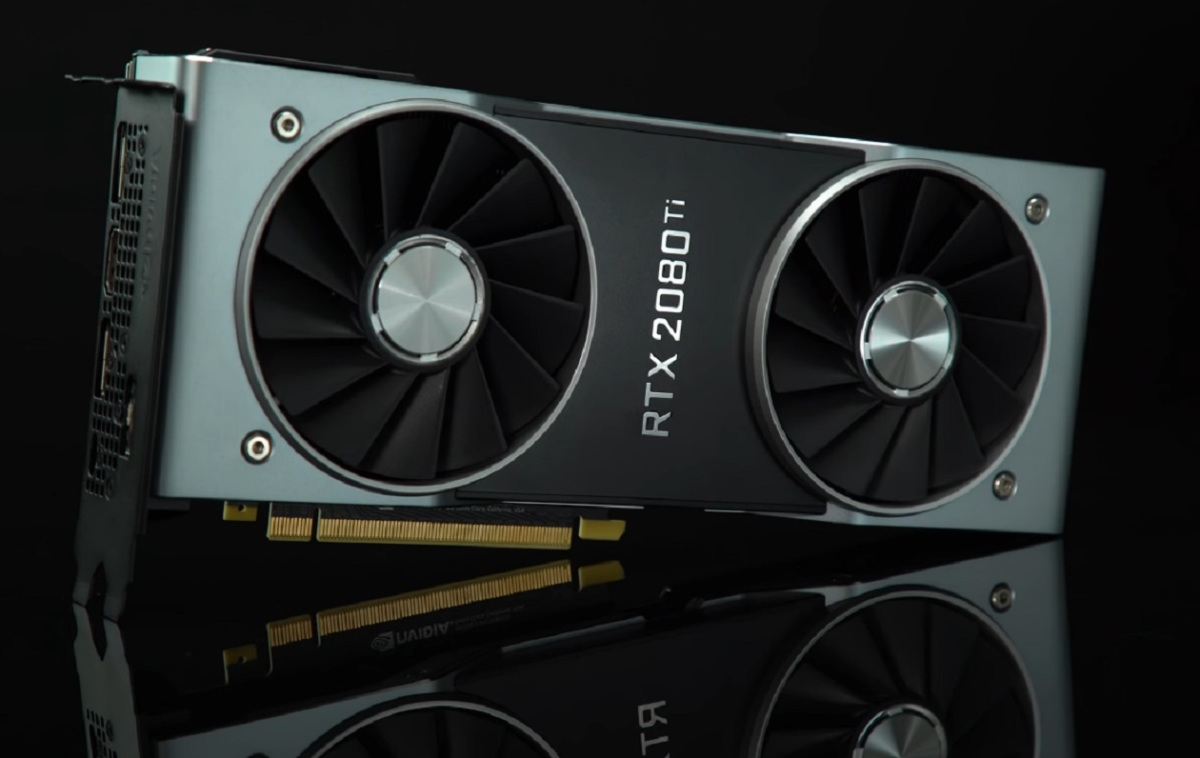
\includegraphics[width=\paperwidth,height=\paperheight]{refs/Nvidia-GeForce-RTX-2080-Ti-1}
%		}
%	} 
    \begin{frame}
    \frametitle{Overview of Product}
        \begin{table}[H]
        \vspace{-0.5cm}
        \hspace{-0.55cm}
        %			\newcolumntype{L}{>{\centering\arraybackslash}m{4cm}}
        \begin{tabular}{ m{4cm} l }
        	{\begin{figure}[H]
        			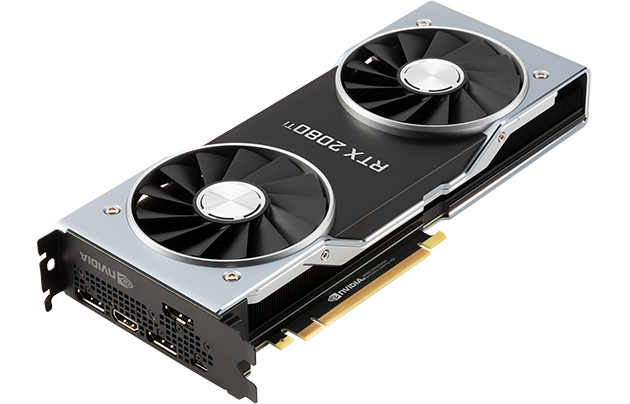
\includegraphics[width=100px]{refs/geforce-rtx-2080-ti-web-tech-shot-630-u}
        			\caption{{\footnotesize RTX 2080 Ti}}
        	\end{figure}}
        	&
        	\makecell{ 
        		14.2 TFLOPS\footnote[1]{Based on peak single precision of GPU boost clock\label{note1}} of FP32
        		\\ 113.8 Tensor TFLOPS
        		\\ 10 Giga Rays/sec
        		\\ 78 Tera RTX-OPS
        	}
        	\\
        	\vspace{-0.5cm}
        	{\begin{figure}[H]
        			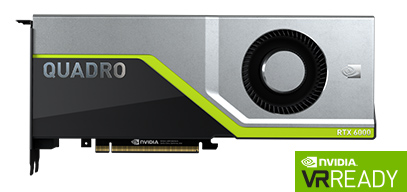
\includegraphics[width=100px]{refs/pre-order-quadro-rtx-6000-front-badge-r2-407-d.jpg}
        			\caption{{\footnotesize QUADRO RTX 6000}}
        	\end{figure}}
        	&
        	\vspace{-0.5cm}
        	\makecell{
        		16.3 TFLOPS\footnotemark[1] of FP32
        		\\ 130.5 Tensor TFLOPS
        		\\ 10 Giga Rays/sec
        		\\ 84 Tera RTX-OPS
        	}
        \end{tabular}
        \end{table}
    \end{frame}

\section{Applications}
    \begin{frame}[allowframebreaks]
    \frametitle{Spectrum of QUADRO}
        \begin{figure}
            \centering
            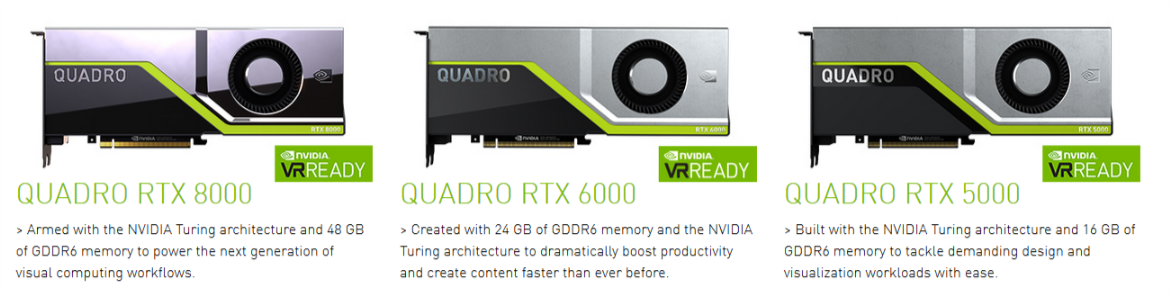
\includegraphics[width=\linewidth]{refs/latest_quadro_rtx_lineup.png}
            \caption{Quadro RTX Line up}
        \end{figure}
        \begin{block}{
            \begin{figure}[H]
            	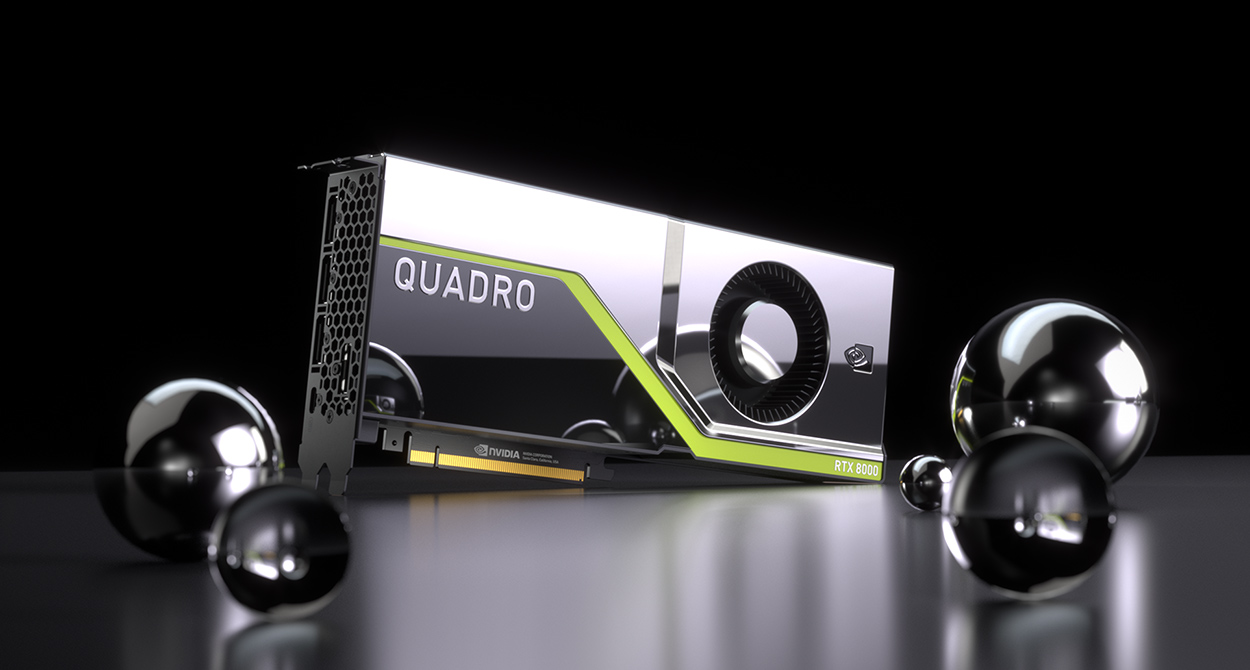
\includegraphics[width=150px]{refs/quadro-design-vis-quadro-rtx-8000-625-u@2x.jpg}
            	\caption{{\footnotesize Quadro in Desktop Workstations}}
            \end{figure}
            }
            {
            Quadro has long been the \gls{de facto standard} for enterprise desktop graphics for digital designers and artists. With a range of performance, capabilities and price points, there is a right Quadro to go with the desktop workstation of your choice.
            }
        \end{block}
        \begin{block}{
            \begin{figure}[H]
            	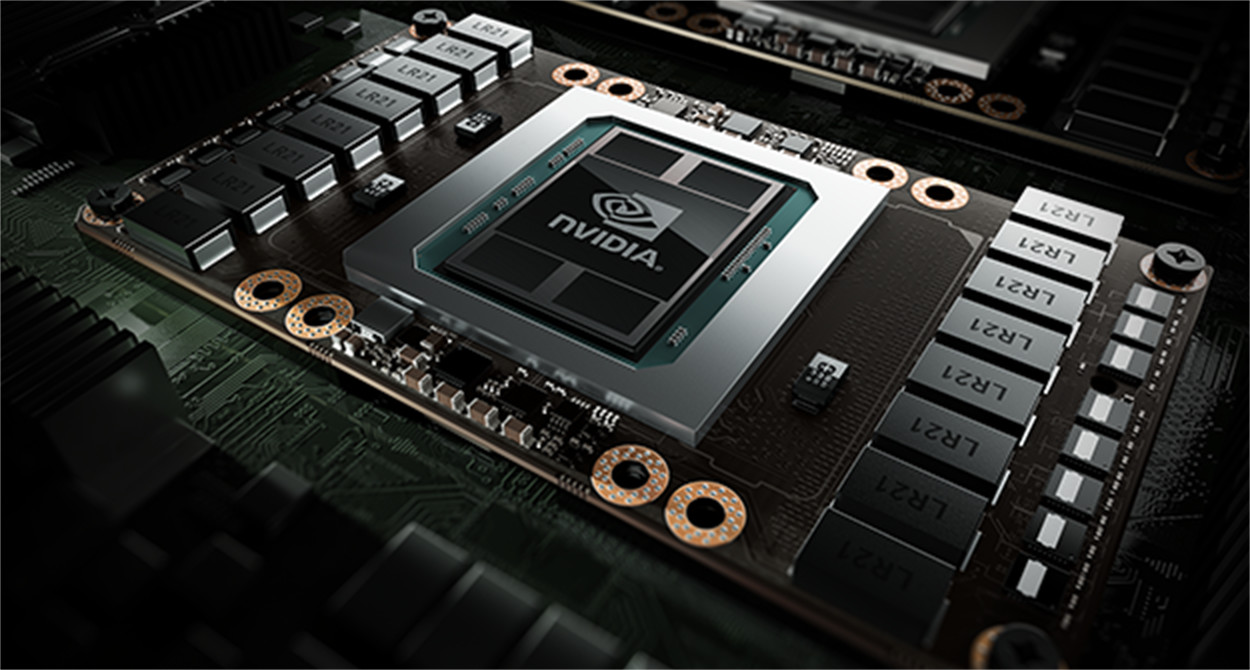
\includegraphics[width=150px]{refs/quadro-whats-new-feature-mobile-625-ud@2x.jpg}
            	\caption{{\footnotesize Quadro in Mobile Workstation}}
            \end{figure}
            }
            {
                Quadro brings desktop-class performance to mobile workstations to enable incredibly powerful, thin and light form factors. Enjoy the ultimate creative freedom - tackle complex datasets with ease, render photorealistic images interactively and develop life-like VR experiences on-the-go.
            }
        \end{block}
        \begin{block}{
            \begin{figure}[H]
            	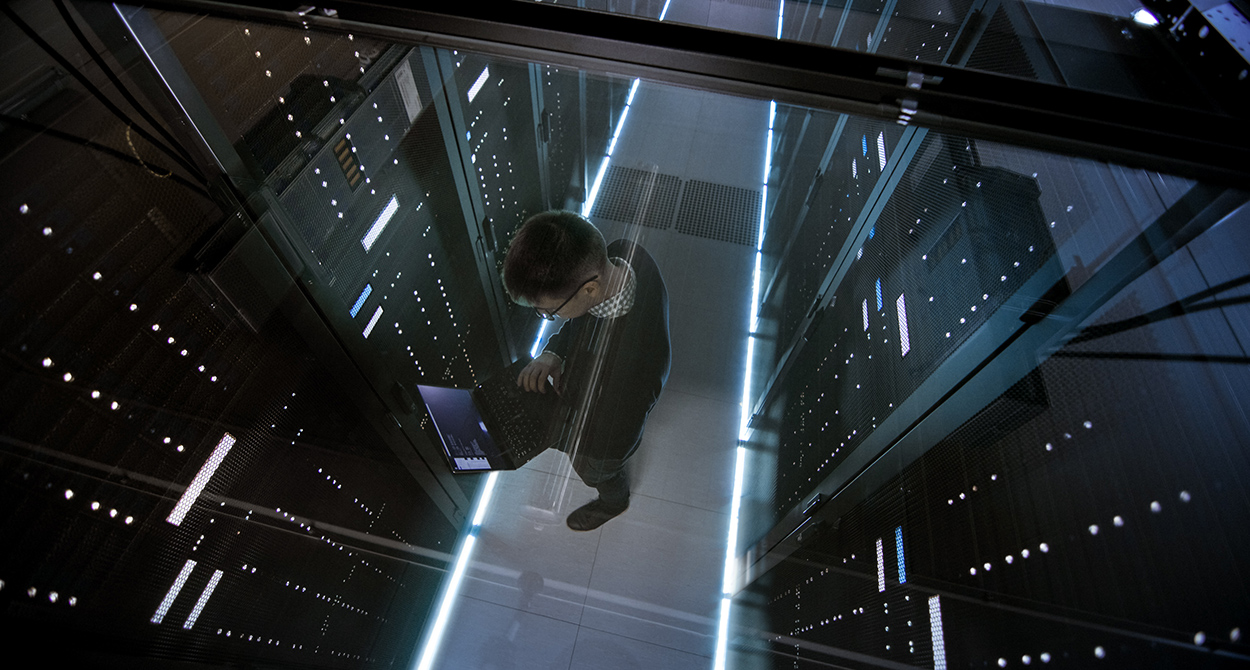
\includegraphics[width=150px]{refs/design-vis-quadro-in-server-625-u@2x.jpg}
            	\caption{{\footnotesize Quadro in Servers}}
            \end{figure}
            }
            {
                There are many complex visual computing workloads that require significantly higher levels of GPU horsepower for performance and efficiency. Quadro is available in industry-leading server solutions so you can scale-up from the desktop to the data center to meet your most demanding needs.
            }
        \end{block}
        \begin{block}{
            \begin{figure}[H]
            	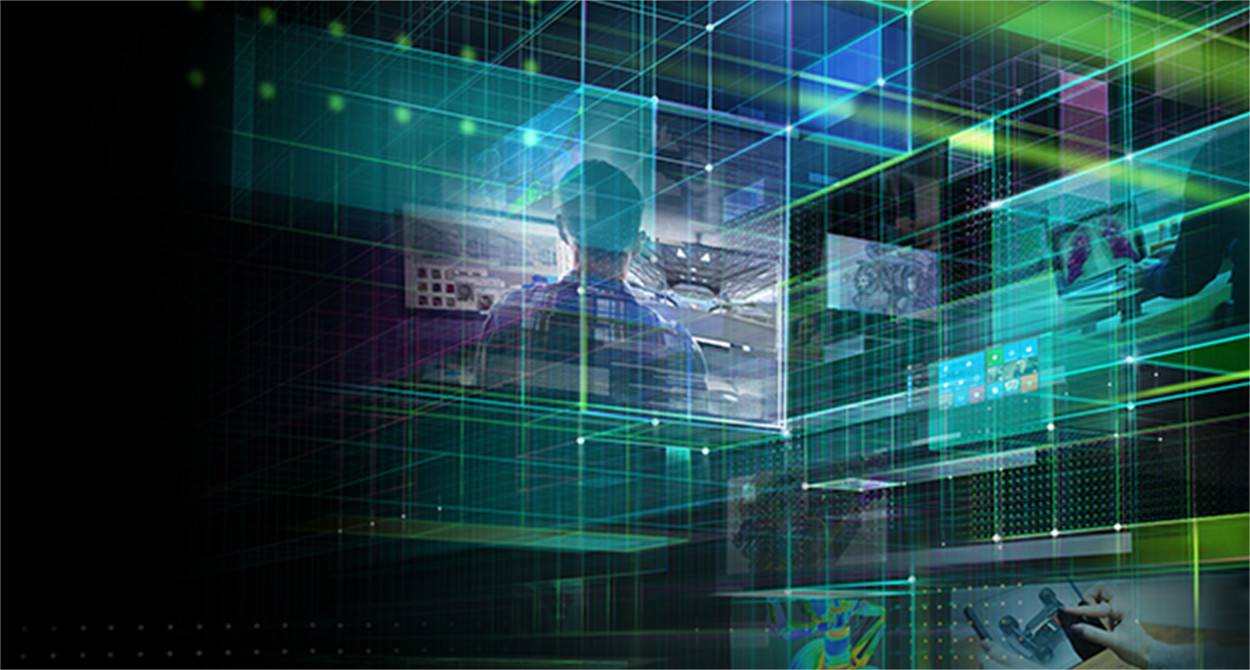
\includegraphics[width=150px]{refs/quadro-whats-new-feature-vdws-625-ud@2x.jpg}
            	\caption{{\footnotesize Quadro in Virtual Workspaces}}
            \end{figure}
            }
            {
                Quadro Virtual Data Center Workstation (Quadro vDWS) provides creative and technical professionals with access from anywhere, and on any device while ensuring the proven performance of traditional Quadro solutions. Virtualized from the data center, the Quadro vDWS delivers a secure, immersive, agile workspace and supports the most demanding professional design and engineering applications.
            }
        \end{block}
        \begin{block}{
            \begin{figure}[H]
            	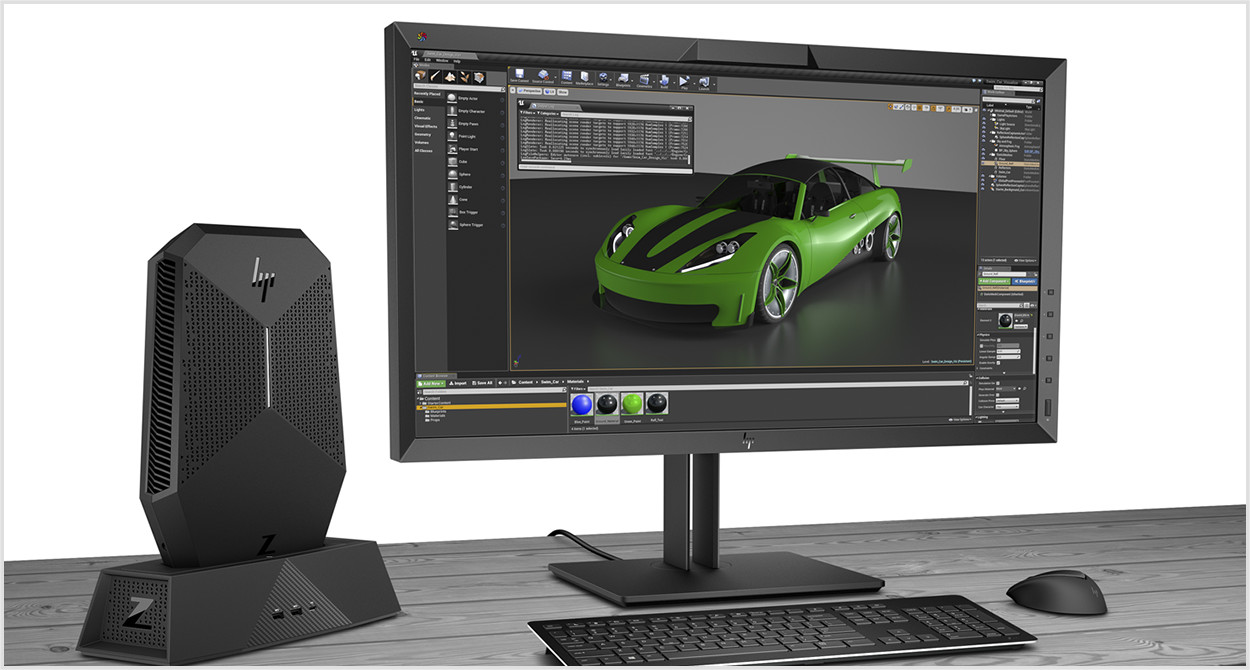
\includegraphics[width=150px]{refs/quadro-whats-new-feature-specialty-625-ud@2x.jpg}
            	\caption{{\footnotesize Quadro in Speciality Solutions}}
            \end{figure}
            }
            {
                Tap into the power of Quadro within innovative solutions that go beyond traditional desktop and mobile form factors. Tablets, backpacks and mini workstations with Quadro under the hood are ideal for professionals who desire full-size workstation performance and application compatibility in purpose-built solutions.
            }
        \end{block}


    \end{frame}


\section{Comparing with Predecessor}
    \begin{frame}{Overview the New}
        \begin{itemize}
            \item New RT (Ray Tracing) Core per SM
            \item Turing SM Architecture (streaming multi-processor design that delivers greater processing efficiency)
            \item Dynamic Parallelism (GPU dynamically spawns new threads without going back to the CPU)
            \item Mixed-precision (1-, 4-, 8-, 16-, 32- and 64-bit) computing
            \item Error correction codes (ECC) on graphics memory
            \item Configurable up to 96 KB of RAM (dedicated shared memory size per SM)
        \end{itemize}
    \end{frame}
    
    \begin{frame}[allowframebreaks]
    \frametitle{The New Features}
        \begin{block}{RT Cores for Real-Time Ray Tracing}
        {\small helps single GPU to render realistic \textbf{cinematic-quality 3D games, complex professional models} with accurate shadows, reflections, refractions.
        \\ The Turing architecture is armed with dedicated ray-tracing processors called RT Cores that accelerate the computation of how light and sound travel in 3D environments by up to 10 Giga Rays per second.
        \\ \href{https://www.youtube.com/watch?v=LXo0WdlELJk}{EA Project PICA real-time ray tracing demo running on NVIDIA RTX}}
        \end{block}
        
        \begin{block}{Tensor Cores for AI Acceleration}
        {\small Tensor Cores - processors that accelerate deep learning training and inference, providing up to \textbf{500 trillion tensor operations per second}.
        \\ This level of performance dramatically accelerates AI-enhanced features—such as denoising, resolution scaling, and video re-timing—creating applications with powerful new capabilities.}
        \end{block}
        
        \begin{block}{New Streaming Multiprocessor}
        {\small The Turing architecture dramatically improves raster performance over the previous-generation Pascal with an enhanced graphics pipeline and new programmable shading technologies (variable-rate shading, texture-space shading, and multi-view rendering).
        }
        \end{block}
        
        \begin{block}{CUDA For Simulation}
        {\small Turing-based GPUs feature a new streaming multiprocessor (SM) architecture that supports \textbf{up to 16 trillion floating-point operations} in parallel with 16 trillion integer operations per second. 
        \\ Developers can take advantage of up to 4,608 CUDA cores with NVIDIA CUDA 10, FleX, and PhysX software development kits (SDKs) to create complex simulations, such as particle or fluid dynamics for scientific visualization, virtual environments, and special effects.}
        \end{block}
    \end{frame}

    \begin{frame}[allowframebreaks]
    \frametitle{Ray Tracing}
    Turing improves Ray tracing up to 6X compared to Volta
    \centering
        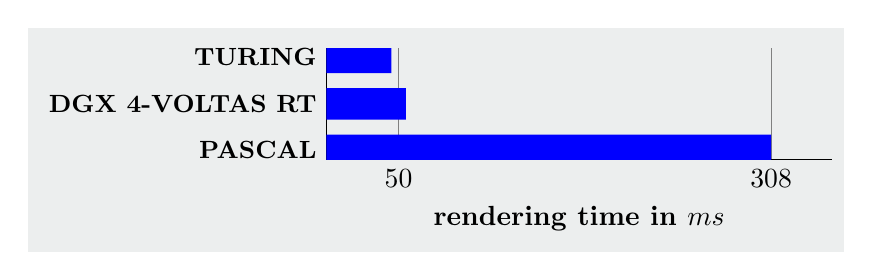
\begin{tikzpicture}[use background]
            \pgfplotstableread[row sep=\\]{ % Read the data into a table macro
            Label                                      		First   Second\\
            {PASCAL}										0     	308\\
            {DGX 4-VOLTAS RT}                               0     	55\\
            {TURING}                         				0     	45\\
            }
            \datatable
            \begin{axis}[
                xbar stacked,   % Stacked horizontal bars
                xmin=0,  xmax=350,       % Start x axis at 0
                %				title={\large \textbf {Gantt Chart }},
                height=3cm, width=8cm,
                bar width=0.4cm,
                axis x line*=bottom,
                axis y line*=left,
                y axis line style={opacity=1},
                enlarge y limits=true,
                xmajorgrids={true},
                grid style={solid,ultra thin,gray},
                tick style={tickwidth=0cm,major tick length=0cm},
                xlabel={\textbf{rendering time in $ ms $}},
                xtick ={50,308},
                yticklabel style={font=\small\bfseries},
                ytick=data,     % Use as many tick labels as y coordinates
                yticklabels from table={\datatable}{Label}  % Get the labels from the Label column of the \datatable
                ]
                \addplot [draw=none,fill=blue] table [x=First, y expr=\coordindex] {\datatable};    % Plot the "First" column against the data index
                \addplot [draw=none,fill=blue]table [x=Second, y expr=\coordindex] {\datatable};
            \end{axis}
        \end{tikzpicture}
        
        \begin{figure}
            \centering
            	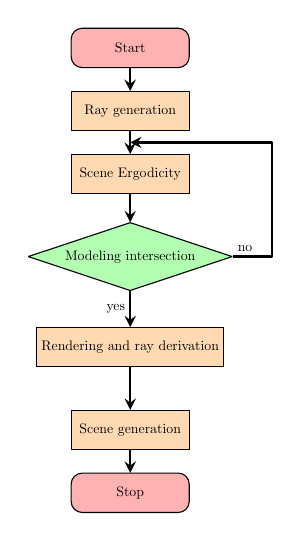
\begin{tikzpicture}[>=latex',line join=bevel, node distance=1.6cm, scale=0.5, every node/.style={transform shape}]
		            \node (start) [startstop] {Start};
		            \node (rayGeneration) [process, below of=start] 
			            {Ray generation};
		            \node (sceneErgodicity) [process, below of=rayGeneration] 
			            {Scene Ergodicity};
			        \node (intersect) [decision, below of=sceneErgodicity, yshift=-0.5cm, aspect=3]
			            {Modeling intersection};
		            \node (rendering) [process, below of=intersect, yshift=-0.7cm, aspect=3]
			            {Rendering and ray derivation};
		            \node (sceneGeneration) [process, below of=rendering, yshift=-0.5cm, aspect=3]
			            {Scene generation};
		            \node (stop) [startstop, below of=sceneGeneration] {Stop};
			        \draw [arrow] (start) -- (rayGeneration);
			        \draw [arrow] (rayGeneration) -- (sceneErgodicity);
			        \draw [arrow] (sceneErgodicity) -- (intersect);
			        \draw [arrow] (intersect.east) node[above right]{no} -- ++ (1,0) |- ($(rayGeneration)!0.5!(sceneErgodicity)$);
			        \draw [arrow] (intersect) -- node[anchor=east] {yes} (rendering);
			        \draw [arrow] (rendering) -- (sceneGeneration);
			        \draw [arrow] (sceneGeneration) -- (stop);
	            \end{tikzpicture}
            \caption{Ray Tracing Base Flow}
            \label{fig:rayTracingFlow}
        \end{figure}
        
        \begin{itemize}
            \item Establish 2-D \textit{kd-tree} structure to store scene information.
            Each node in tree stands for axis-aligned bounding box and every inner node represents separation plane which divides the scene into two sub-regions
            \item change the order clue into threaded binary-tree before calculating intersection and ergodicity.
            \item if the ray's span crosses two sides of the separation axles, that ray goes through two second-level boxes at the same time so we will first calculate its intersection with the first child node.
            \item if that node is a leaf node, and the reflection has intersection with that node, the result will be a success. Otherwise, successor nodes of that node will be searched directly.
        \end{itemize}
        
        % \newpage
        % \begin{equation}
        %     C(n) = \sum_{j=1}^{n}M_j(\Pi_{i=1}^{j=1}r_i)(1-r_i)
        % \end{equation}
        
        % $C(n)$ final color of pixel - The function of rendering and ray derivation is to figure out the color value
        % \\    
        % $M_j$ model j
        % \\
        % $r_i$ reflection coefficient of object i
                
        \begin{figure}
            \centering
            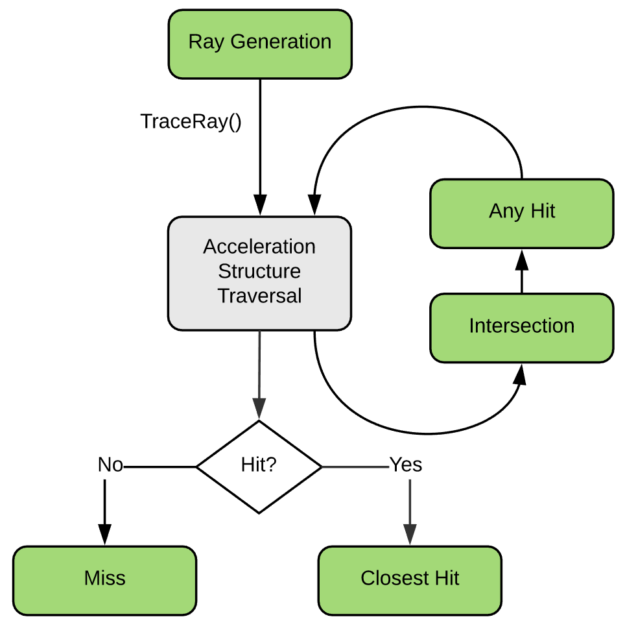
\includegraphics[height=180px]{refs/raytrace_01-625x630.png}
            \caption{Ray Tracing Pipeline}
            \label{fig:rayTracingFlownVidia}
        \end{figure}
        
    \end{frame}

    \begin{frame}[allowframebreaks]
    \frametitle{Comparing Workstation GPU}
    %			\def\arraystretch{1.5}
        \begin{longtable}{c | l | l}
            & \theadfont Quadro RTX 6000 & \theadfont Volta 100
                \\ \hline
            \makecell{CUDA Parallel-\\Processing Cores} & 4608 & 5120
                \\ \hline
            Architecture & Turing & Volta
                \\ \hline
            Code Name & TU102 & GV100
                \\ \hline
            Transistor count & 18,600 million & 21,100 million
                \\ \hline
            Transistors & 12nm & 12nm
                \\ \hline
            \makecell{SMs} & 72 & 80
                \\ \hline
            \makecell{GPU Base \\clock speed} & 1440 MHz & 1132 MHz
                \\ \hline
            \makecell{GPU Boost \\Clock speed} & 1770 MHz & 1530 MHz
                \\ \hline
            \makecell{Memory \\clock speed} & 12000 MHz & 1696 MHz
                \\ \hline
            \makecell{Memory \\Bandwidth} & 624 GB/s & 870 GB/s
                \\ \hline
            \makecell{\gls{tensorcore}} & 576 & 640
                \\ \hline
            \makecell{\gls{rtcore}} & 72 & -
                \\ \hline		
            GPU Memory & 24 GB GDDR6 & 32 GB HBM2
                \\ \hline
            RTX-OPS & 84 Tera-OPS & -
                \\ \hline
            Rays Cast & 10 Giga Rays/Sec & -
                \\ \hline
            \makecell{FP32 \\Performance} & 16.3 TFLOPS & 14.8 TFLOPS
                \\ \hline
            \makecell{Tensor \\Performance\footnote{FP16 matrix multiply with FP16 and FP32 accumulate}} & 130.5 TFLOPS & 118.5 TFLOPS
                \\ \hline
            \makecell{Max Power \\Consumption} & 295 W & 250 W
                \\ \hline
            Graphics Bus & PCI Express 3.0 x 16 & PCI Express 3.0 x 16
                \\ \hline
            \makecell{Display \\Connectors} & \makecell{DP 1.4 (4),\\ VirtualLink (1)} & \makecell{DP 1.4 (4)}
                \\ \hline
            Form Factor & \makecell{4.4" H $\times$ 10.5" L\\ Dual Slot} & \makecell{4.4" H $\times$ 10.5" L \\Dual Slot}
                \\ \hline
            Release date & 13 August 2018 & 27 March 2018
                \\ \hline
            Launch Price & \$6299 & \$8999
        \end{longtable}
    \end{frame}

    \begin{frame}
        \begin{figure}[H]
            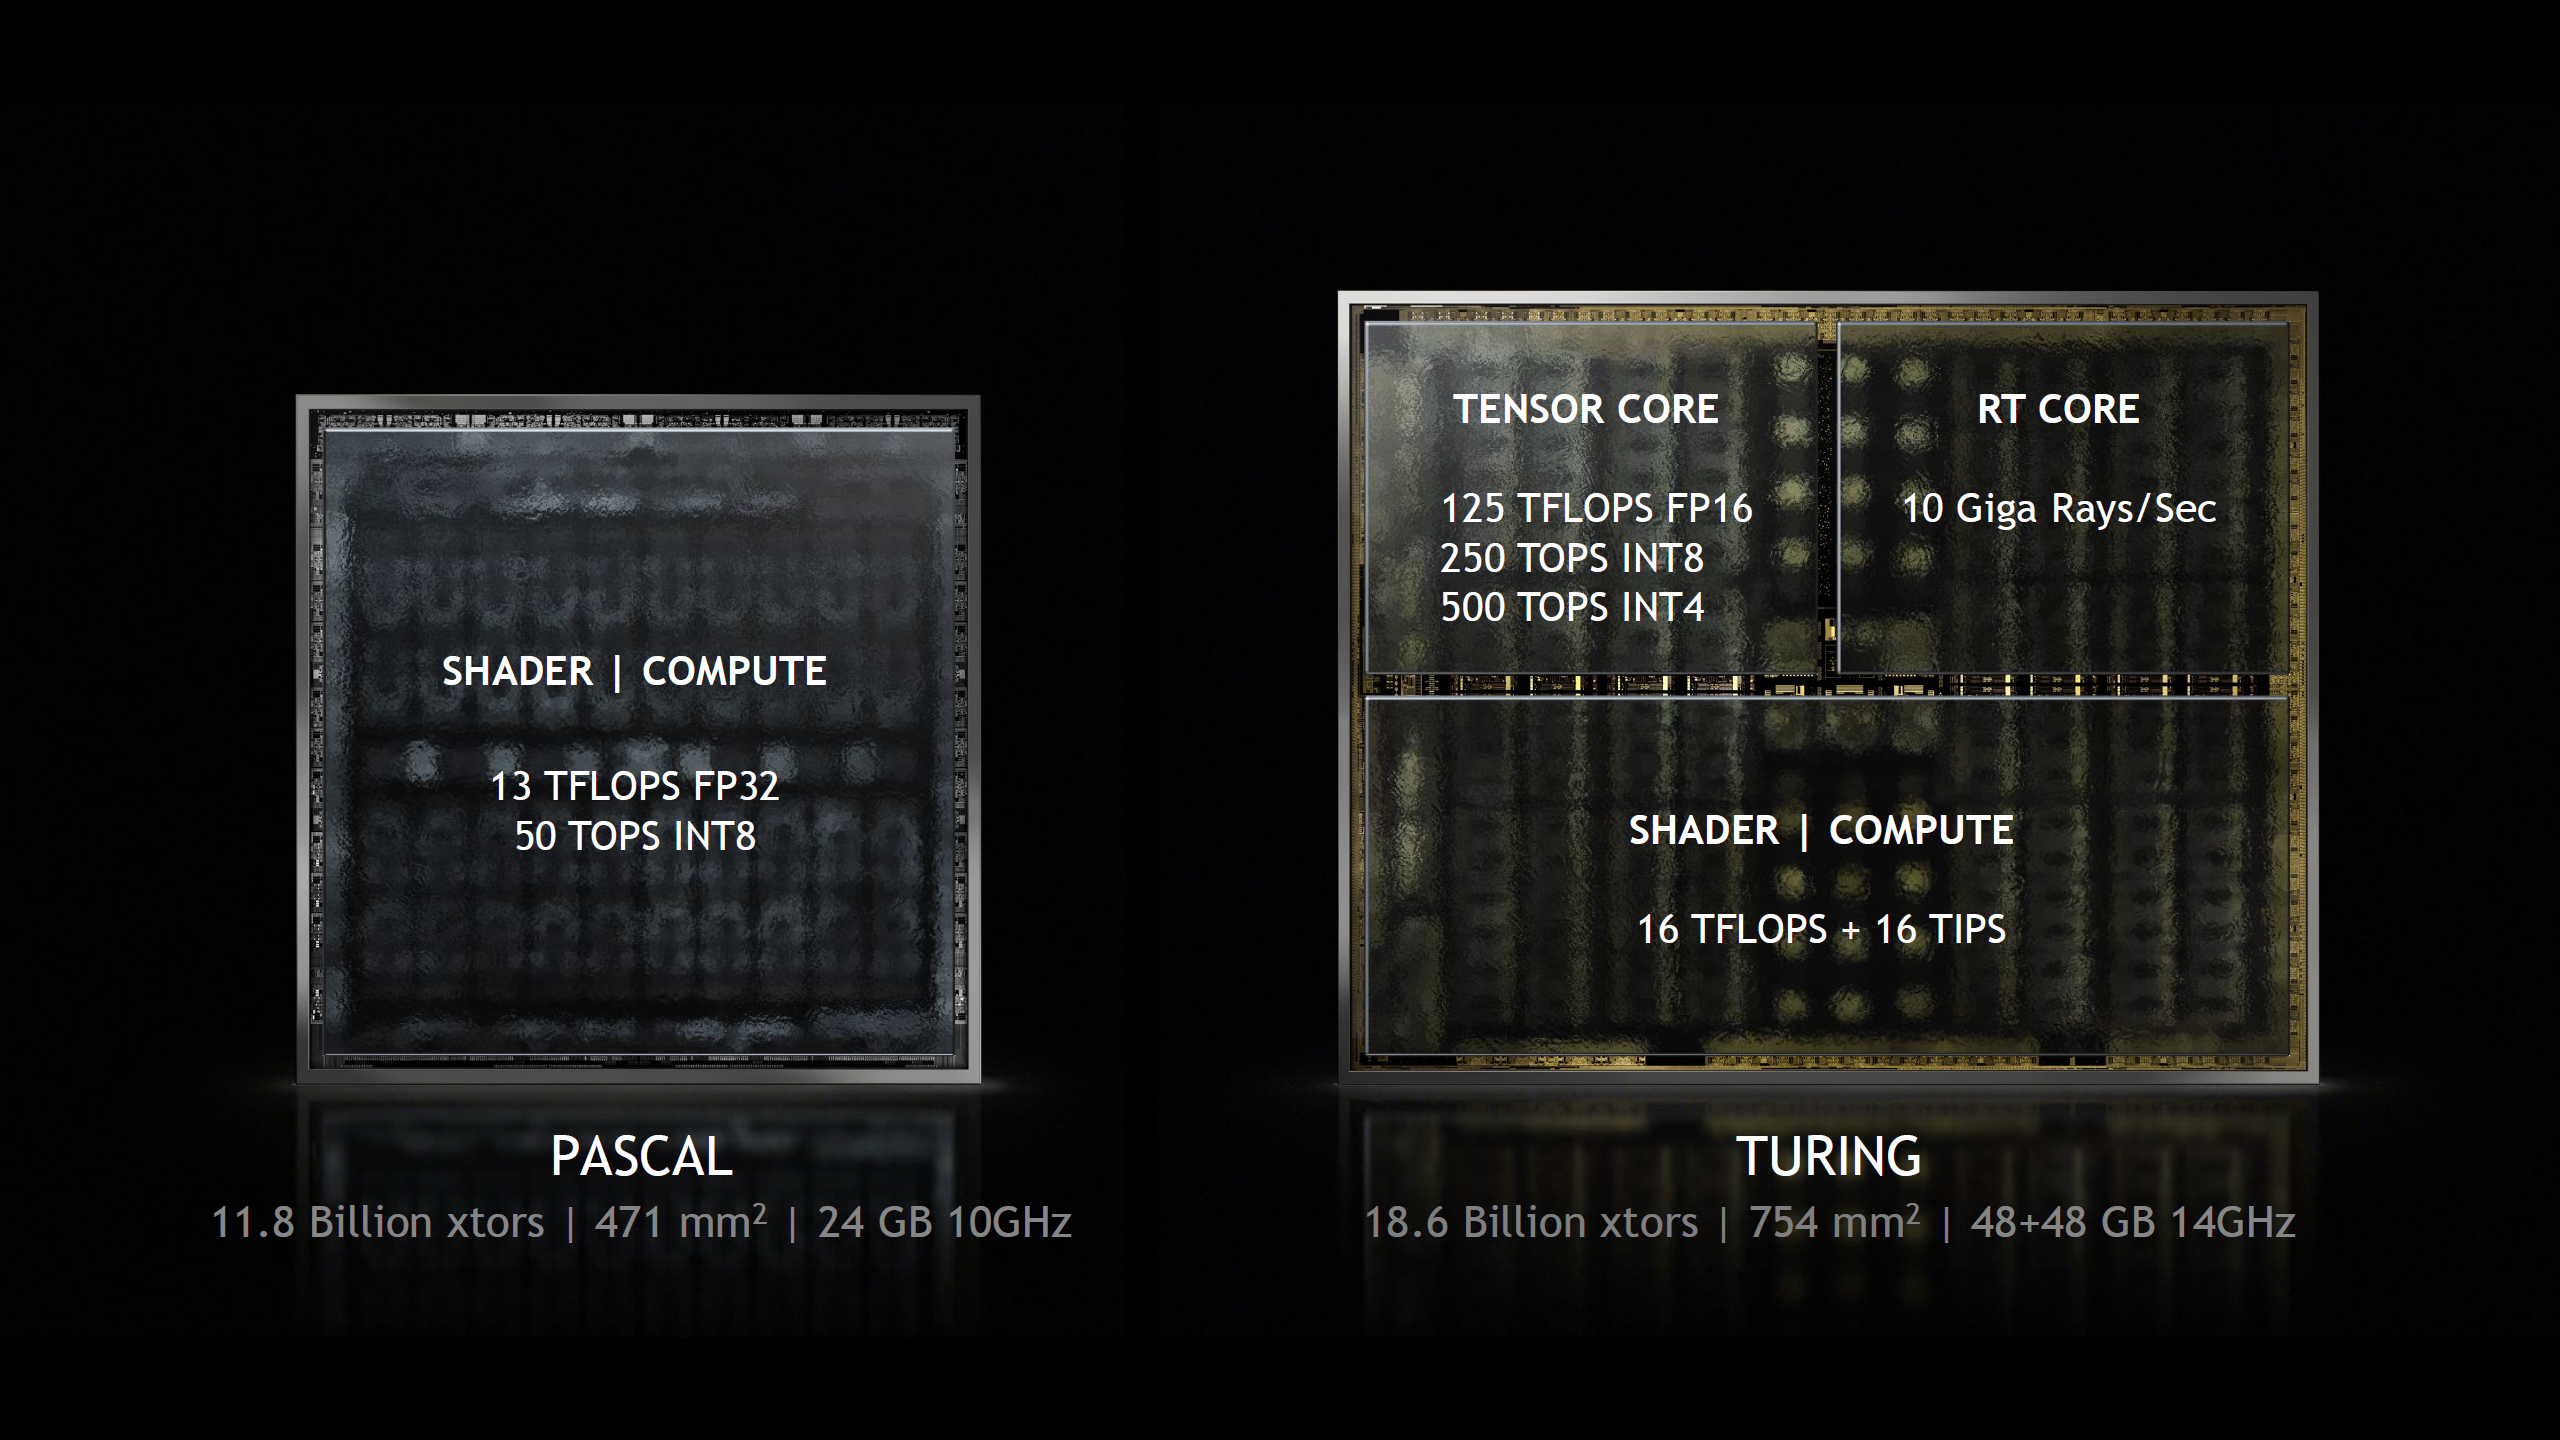
\includegraphics[width=270px]{refs/NVIDIA-RTX-Turing-GPU_19-1}
        \end{figure}
    \end{frame}

\section{In to the Architecture}
    \begin{frame}[allowframebreaks]
    \frametitle{Tensor Core}
        \begin{itemize}
            \item Tesla T4 introduces NVIDIA Turing Tensor Core technology with multi-precision computing for the world’s most efficient AI inference. 
            
            \item Turing Tensor Cores provide a full range of precisions for inference, from FP32 to FP16 to INT8, as well as INT4, to provide giant leaps in performance over NVIDIA Pascal® GPUs.
            
            \item however it's predecessor Nvidia V100 GPU (Volta) having first-generation Tensor Cores can only deliver performance with mixed-precision matrix multiply in FP16 (12X compare to PASCAL) and FP32(6X compare to PASCAL)
        \end{itemize}
        
        \begin{figure}[H]
            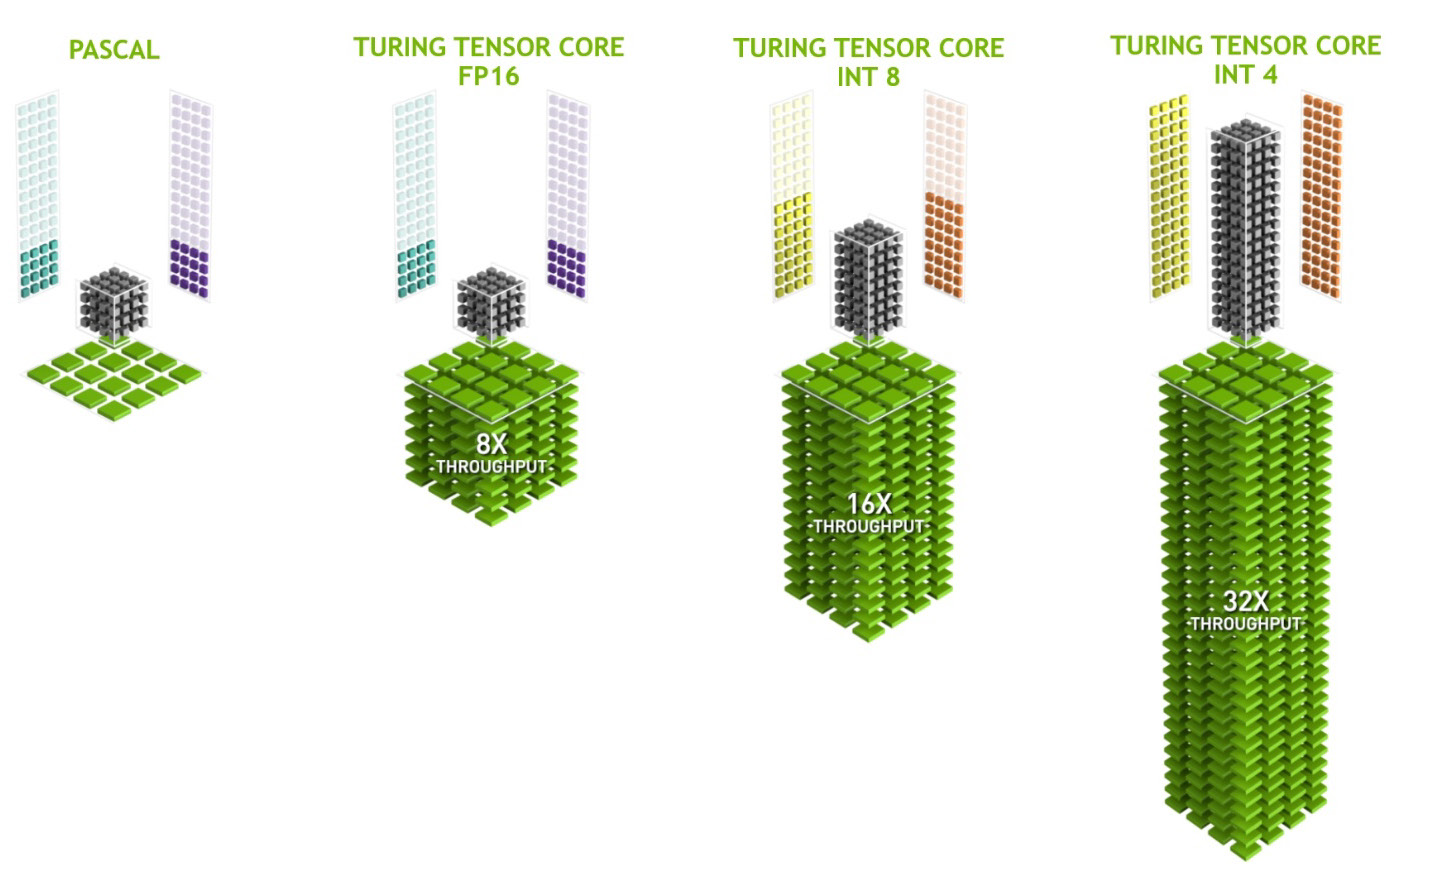
\includegraphics[width=270px]{refs/turing-throughput-tensor.jpg}
            \caption{Turing Tensor core throughput comparison}
        \end{figure}
        
        \begin{figure}
            \centering
            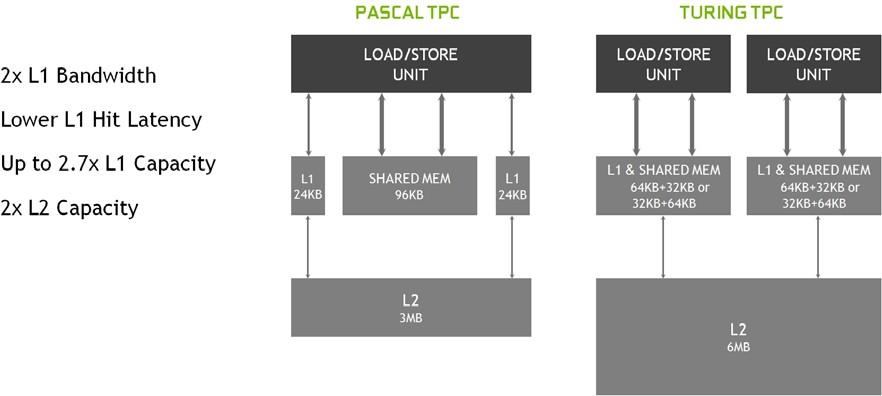
\includegraphics[width=270px]{refs/image3.jpg}
            \caption{New Shared Memory Architecture}
            \label{fig:newSM}
        \end{figure}
    \end{frame}

\section{Terminologies}
    \begin{frame}[allowframebreaks]
    \frametitle{Glossaries}
        \printglossaries
    \end{frame}

    \begin{frame}
    \frametitle{The End}
    \centering
    {\fontsize{40}{50}\selectfont Thank You!}
    \end{frame}
\end{document}